% =============================================================================
% 03-approach.tex  —  Section: Προσέγγιση  (S6–S8, ~3 frames, ~3 min)
% Ξεκινά τη section «Προσέγγιση» — το 04-kernels.tex συνεχίζει στην ίδια section.
% Δομή: ο 3-tier μηχανισμός επιτάχυνσης του polymul σε βάθος
% (Tier 1 scalar Zbc → Tier 2 Base-RVV → Tier 3 Zvbc). Headline speedups:
% polymul HQC-128 Tier1/2/3 = x101.3 / x124.6 / x264.1
% polymul HQC-256 Tier1/2/3 = x110.2 / x133.4 / x436.5
% src: results/reports/summaries/speedups_simulation.md
% =============================================================================
\section{Προσέγγιση}

% --- Frame S6: Tier 1 — scalar Zbc CLMUL + Karatsuba ---
\begin{frame}{\en{Tier~1} — \Zbc \clmul: από bit-serial schoolbook σε word-level (\HL{\speedup{101}})}
  \begin{columns}[T]
    \begin{column}{0.46\textwidth}
      \begin{itemize}
        \item \con{Ρεφ.:} bit-serial schoolbook, $\BigO{N^2}$ shift-and-XOR — \emph{χιλιάδες εντολών/word}
        \item \pos{\Zbc \clmul/\clmulh:} \emph{1 εντολή} για 64-\en{bit} \en{carry-less} γινόμενο στο $\GFpoly$
        \item \HL{\en{Karatsuba}} αναδρομή: $3$ αντί $4$ υπο-γινόμενα ανά επίπεδο — $\BigO{N^{1.585}}$
        \item Καθαρό λογισμικό, μηδέν custom \en{hardware}
        \item \HL{\speedup{101.3}} (\en{HQC-128}), \speedup{110.2} (\en{HQC-256})
      \end{itemize}
    \end{column}
    \begin{column}{0.54\textwidth}
      \centering
      \resizebox{\columnwidth}{!}{%
        % Comparison: bit-serial schoolbook vs word-level clmul leaf
% Used in §6.2.1 (ssec:bit-to-word)

\tikzsetnextfilename{ch6-polymul-schoolbook-vs-clmul}
\begin{tikzpicture}[
  box/.style={draw, rounded corners=2pt, minimum width=4.8cm,
    minimum height=2.2cm, align=left, font=\ttfamily\small},
  arrow/.style={->, thick, >=stealth},
  label/.style={font=\sffamily\small\bfseries, above}
]

% Left box: bit-serial schoolbook
\node[box, fill=red!5] (school) at (0,0) {%
  \begin{tabular}{@{}l@{}}
  for i in 0..n-1:\\
  \quad for bit in 0..63:\\
  \quad\quad mask = -(a[i]>>bit \& 1)\\
  \quad\quad for j in 0..n-1:\\
  \quad\quad\quad r[i+j] \^{}= (b[j]<<bit) \& mask\\
  \quad\quad\quad r[i+j+1] \^{}= (b[j]>>inv) \& mask
  \end{tabular}
};
\node[label] at (school.north) {Bit-serial schoolbook};
\node[font=\sffamily\footnotesize, below=2pt] at (school.south)
  {$64 \times n^2$ conditional shift-XOR};

% Right box: clmul leaf
\node[box, fill=green!5] (clmul) at (7.5,0) {%
  \begin{tabular}{@{}l@{}}
  for i in 0..n-1:\\
  \quad for j in 0..n-1 (pairs):\\
  \quad\quad lo = clmul(a[i], b[j])\\
  \quad\quad hi = clmulh(a[i], b[j])\\
  \quad\quad r[i+j] \^{}= lo\\
  \quad\quad r[i+j+1] \^{}= hi
  \end{tabular}
};
\node[label] at (clmul.north) {Word-level \textsf{Zbc} leaf};
\node[font=\sffamily\footnotesize, below=2pt] at (clmul.south)
  {$n^2$ ζεύγη clmul/clmulh};

% Arrow between
\draw[arrow, very thick, color=blue!60!black]
  (school.east) -- node[above, font=\sffamily\small] {$\times$64}
  (clmul.west);

\end{tikzpicture}
%
      }
    \end{column}
  \end{columns}
  \pnote{60 s. Frame 6. Tier 1 = scalar clmul leaf + Karatsuba split. One instruction replaces the inner shift-XOR loop. Land the x101.}
\end{frame}

% --- Frame S7: Tier 2 — Base-RVV vectorization (no Zvbc) ---
\begin{frame}{\en{Tier~2} — \en{Base-RVV}: διανυσματοποίηση \emph{χωρίς} \Zvbc (\HL{\speedup{125}})}
  \begin{columns}[T]
    \begin{column}{0.50\textwidth}
      \begin{itemize}
        \item Ιδέα: πολλαπλά \en{limbs} ανά \en{vector} λειτουργία — \en{data-level parallelism}
        \item \HL{\en{Strip-mining}} με \VLMAX/\LMUL: αυτόματος χειρισμός μέγεθους
        \item \en{Vectorized} schoolbook: \en{vector shifts} + \en{XOR} (\Zvbb \vror)
        \item \emph{Χωρίς} \en{carry-less} υλικό — αμιγώς \en{base} \RVV ως baseline
        \item \HL{\speedup{124.6}} (\en{HQC-128}), \speedup{133.4} (\en{HQC-256})
      \end{itemize}
    \end{column}
    \begin{column}{0.50\textwidth}
      \centering
      \resizebox{\columnwidth}{!}{%
        % VARIANT — not \input by main.tex; promote manually
% rvv-strip-mining_twotone.tex — alternative colour strategy: a clean two-hue
%   alternation between consecutive iterations (emphasises iteration BOUNDARIES
%   rather than per-iteration identity). Remainder still tail-tinted. Tokens only.
\tikzsetnextfilename{ch3-riscv-rvv-strip-mining_twotone}
\begin{tikzpicture}[
  cell/.style={draw=figrule, figLW/hair, minimum width=0.45cm, minimum height=0.5cm,
               font=\ttfamily\tiny, inner sep=0pt},
  lbl/.style={figT/label},
  micro/.style={figT/annot},
  count/.style={figT/annot, anchor=west},
  mbrace/.style={decorate, figLW/base, draw=figrule,
                 decoration={brace, amplitude=4pt, mirror, raise=1pt}},
  even/.style={fill=figprocess!24}, odd/.style={fill=figaccent!24},
  tail/.style={fill=figthreat!22},
]
% === VLMAX = 4 (top) ===
\node[lbl, anchor=west] at (-1.6, 0.8) {\textbf{VLMAX = 4}\ \ (\VLEN=256, SEW=64, LMUL=1)};
\foreach \i in {0,...,19} {
  \pgfmathsetmacro{\xpos}{\i * 0.5}
  \pgfmathtruncatemacro{\grp}{int(\i/4)}
  \ifodd\grp \node[cell, odd] at (\xpos, 0) {\i};
  \else \node[cell, even] at (\xpos, 0) {\i};\fi
}
\foreach \start in {0,2,4,6,8} {
  \draw[mbrace] (\start-0.2, -0.4) -- (\start+1.6, -0.4)
    node[midway, below=3pt, micro] {vl=4};
}
\node[count] at (10.0, 0) {5 iterations};

% === VLMAX = 8 (bottom) ===
\node[lbl, anchor=west] at (-1.6, -2.0) {\textbf{VLMAX = 8}\ \ (\VLEN=512, SEW=64, LMUL=1)};
\foreach \i in {0,...,19} {
  \pgfmathsetmacro{\xpos}{\i * 0.5}
  \ifnum\i>15
    \node[cell, tail] at (\xpos, -2.8) {\i};
  \else
    \pgfmathtruncatemacro{\grp}{int(\i/8)}
    \ifodd\grp \node[cell, odd] at (\xpos, -2.8) {\i};
    \else \node[cell, even] at (\xpos, -2.8) {\i};\fi
  \fi
}
\draw[mbrace] (-0.2, -3.2) -- (3.6, -3.2) node[midway, below=3pt, micro] {vl=8};
\draw[mbrace] (3.8, -3.2) -- (7.6, -3.2) node[midway, below=3pt, micro] {vl=8};
\draw[mbrace, draw=figthreat, figLW/emph] (7.8, -3.2) -- (9.6, -3.2)
  node[midway, below=3pt, micro, text=figthreat!80!black] {vl=4 (remainder)};
\node[count] at (10.0, -2.8) {3 iterations};
\end{tikzpicture}
%
      }
    \end{column}
  \end{columns}
  \pnote{55 s. Frame 7. Tier 2 = base RVV, no Zvbc. Strip-mining over LMUL groups. Modest gain over Tier 1 but it's the vector scaffold for Tier 3.}
\end{frame}

% --- Frame S8: Tier 3 — Zvbc vectorized carry-less multiply ---
\begin{frame}{\en{Tier~3} — \Zvbc \vclmul: διανυσματικό \en{carry-less} γινόμενο (\HL{\speedup{264}})}
  \begin{columns}[T]
    \begin{column}{0.48\textwidth}
      \begin{itemize}
        \item \pos{\Zvbc \vclmul/\vclmulh:} \en{carry-less} γινόμενο σε \emph{ολόκληρο} \en{vector} ταυτόχρονα
        \item Συνδυασμός \en{Karatsuba} $+$ \en{vectorized} φύλλα: το καλύτερο από τις δύο προσεγγίσεις
        \item Πλήρης αποσυμπλοκή από το \en{scalar critical path}
        \item Κλιμακώνει με \VLEN: μεγαλύτερο όφελος στο \en{HQC-256}
        \item \HL{\speedup{264.1}} (\en{HQC-128}), \HL{\speedup{436.5}} (\en{HQC-256})
      \end{itemize}
    \end{column}
    \begin{column}{0.52\textwidth}
      \centering
      \resizebox{\columnwidth}{!}{%
        % AP-2 Generator Pipeline diagram
% Used in §6.2.3 (ssec:ap2-generator)

\tikzsetnextfilename{ch6-polymul-ap2-pipeline}
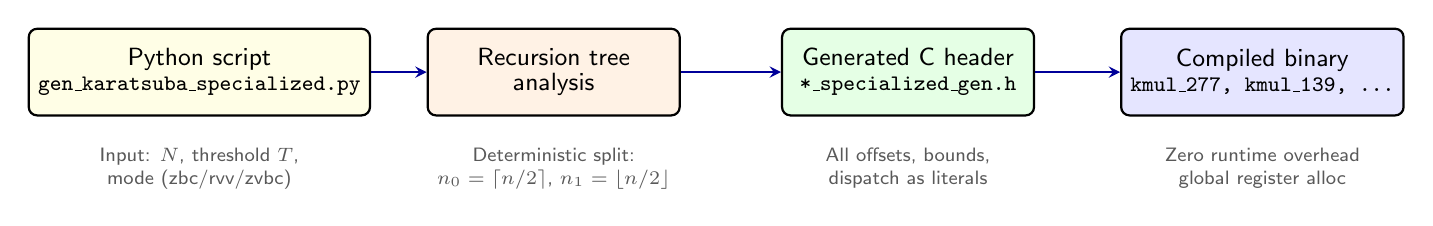
\begin{tikzpicture}[
  stage/.style={draw, rounded corners=3pt, minimum width=3.2cm,
    minimum height=1.1cm, align=center, font=\sffamily\small, thick},
  arrow/.style={->, thick, >=stealth, color=blue!60!black},
  note/.style={font=\sffamily\scriptsize, text=gray!70!black, align=center}
]

% Stage 1: Python script
\node[stage, fill=yellow!10] (script) at (0,0)
  {Python script\\[-2pt]\texttt{\footnotesize gen\_karatsuba\_specialized.py}};

% Stage 2: Recursion tree analysis
\node[stage, fill=orange!10] (tree) at (4.5,0)
  {Recursion tree\\[-2pt]analysis};

% Stage 3: Generated C header
\node[stage, fill=green!10] (header) at (9,0)
  {Generated C header\\[-2pt]\texttt{\footnotesize *\_specialized\_gen.h}};

% Stage 4: Compiled binary
\node[stage, fill=blue!10] (binary) at (13.5,0)
  {Compiled binary\\[-2pt]\texttt{\footnotesize kmul\_277, kmul\_139, \ldots}};

% Arrows
\draw[arrow] (script) -- (tree);
\draw[arrow] (tree) -- (header);
\draw[arrow] (header) -- (binary);

% Annotations below
\node[note, below=8pt] at (script.south) {Input: $N$, threshold $T$,\\mode (zbc/rvv/zvbc)};
\node[note, below=8pt] at (tree.south) {Deterministic split:\\$n_0 = \lceil n/2 \rceil$, $n_1 = \lfloor n/2 \rfloor$};
\node[note, below=8pt] at (header.south) {All offsets, bounds,\\dispatch as literals};
\node[note, below=8pt] at (binary.south) {Zero runtime overhead\\global register alloc};

\end{tikzpicture}
%
      }
    \end{column}
  \end{columns}
  \pnote{60 s. Frame 8. Tier 3 = Zvbc vclmul, the payoff. One carry-less multiply across the whole vector; combined with Karatsuba. Scales with VLEN -> bigger win on HQC-256 (x436).}
\end{frame}
